\section{Dependability}
  \label{sec:Dependability}
  In his book \textit{Software Engineering}, Ian Sommerville describes the term dependability to mean \textit{'The dependability of a computer system 
  is a property of the system that reflects its trustworthiness.'} [28]. He the breaks this down into 4 sections which I will now discuss.

  \begin{figure}[H]
    \centering
    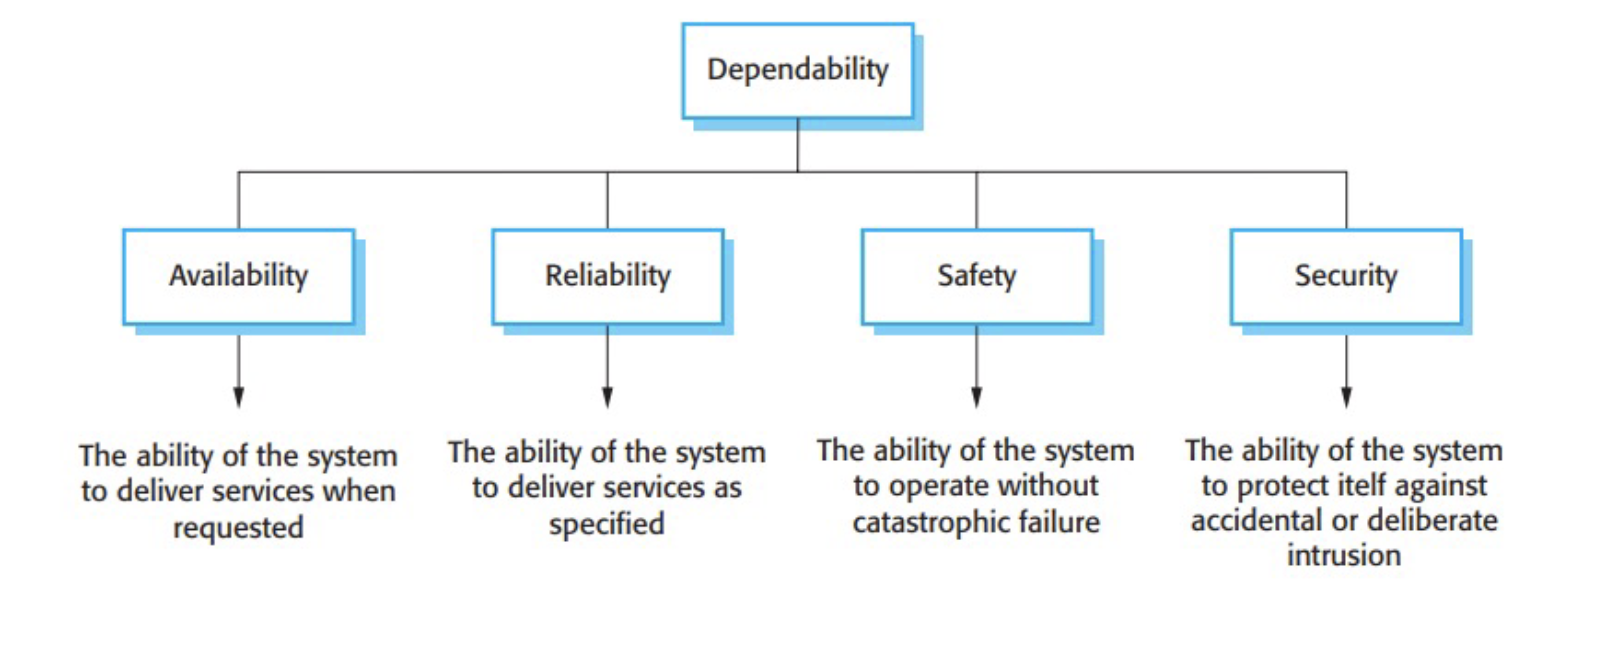
\includegraphics[width=12cm]{assets/dependability.png}
    \caption{Diagram showing the different parts of dependability [28].}
    \label{fig:dependability}
  \end{figure}

  \subsection{Reliability}
  Availability and reliability are closely linked. The image below describes the difference.
  \begin{figure}[H]
    \centering
    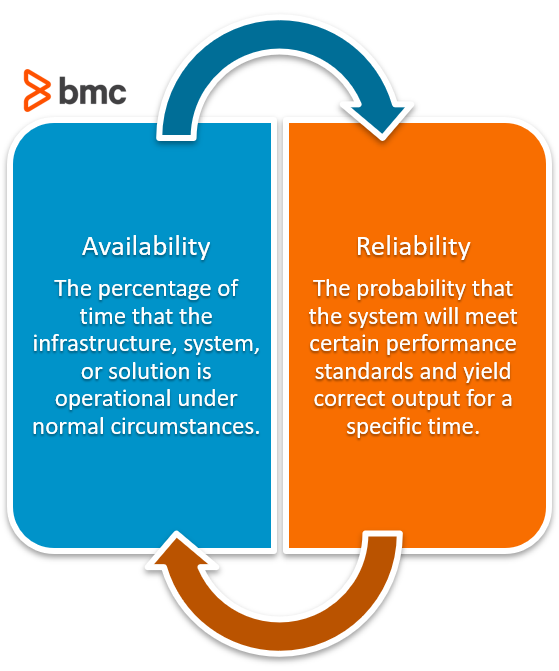
\includegraphics[width=5cm]{assets/avail-reliab.png}
    \caption{Diagram showing the difference between availability and reliability [29].}
    \label{fig:availabilityVsReliability}
  \end{figure}

  \subsubsection{Metric for ACME system reliability}

  The web app is the highest priority and needs to successfully service as many customers as possible.
  I have chosen the metric \textbf{POFOD = 0.0001} meaning that it is acceptable for the service to be unavailable once every 1000 requests. As this is a 
  cloud-native approach ACME has no control over what AWS will do. They themselves will have systems in place to counteract this however for 99.9\% of
  requests to succeed is still high availability.

  To measure this requirement AWS can help us once again. AWS provides metrics for it's components. For the web app we can check the status code
  metric, if the user receives a 5** this is a server error, otherwise known as downtime. We can then use this data to check the amount of requests that 
  have failed due to internal server errors and check it against the metric.

  \subsection{Fault tolerance}
  Other than third party issues there are security problems that could arise. The first thing to tackle is the code itself, the code should be written in 
  a memory safe language. Non-memory safe languages (such as C) allow programmers direct access to memory which can result in attacks such as buffer
  overflows and use-after-free attacks [30]. I would recommend Python due its vibrant community and an older study showed
  that the total code written and time spent writing was the lowest out of a handful of other languages [31].

  Ian Sommerville outlines 8 steps for dependable programming guidelines [28].

  \begin{enumerate}
    \label{sec:PoLP}
    \item \textit{Limit the visibility of information in a programme} - This can be linked to the Principle of Least Privilege (PoLP) idea which 
    \textit{'refers to an information security concept in which a user is given the minimum levels of access' [32]}. Users, both internal and external, 
    should only have access to what they need to access to do their jobs. 

    However this can also be extended in a cloud-native architecture so that the individual components of the system only need permission to access what 
    they need to function. For example the payment lambda does not need access to the account lambda. This not only breaks PoLP, but also the idea of
    microservices being self-contained operations. Steps and processes should be in place to both staff and code to revoke permissions that are no
    longer needed.

    \item \textit{Check all inputs for validity} - This is vital for two reasons. The first is data integrity, you may have a schema that you want users
    data to conform to. This can make querying data easier, but also save money as you won't be having to pay for extra data storage. Additional checks such 
    as size and range checks [28] should be done, and helpful error messages returned to the client.
    
    However the main reason is security. In OWASPs' top 10 vulnerabilities list [33] \textit{'Injection'} is 3rd and covers both XSS (Cross Site Scripting) 
    and SQL injection attacks. These are nearly always exploited via unsanitised inputs. Both client and server-side checks must be made on any data
    provided by the user. 

    \item \textit{Provide a handler for all exceptions} - This is achieved by try/catch/finally statements, or the alternative in other languages. If an 
    error occurs but is not caught, then the system could fail. In addition to this catching the error also provides an opportunity for monitoring and 
    finding potential defects in the system. Below shows the code difference between a correctly handled error and not.

    \begin{figure}[H]
      \centering
      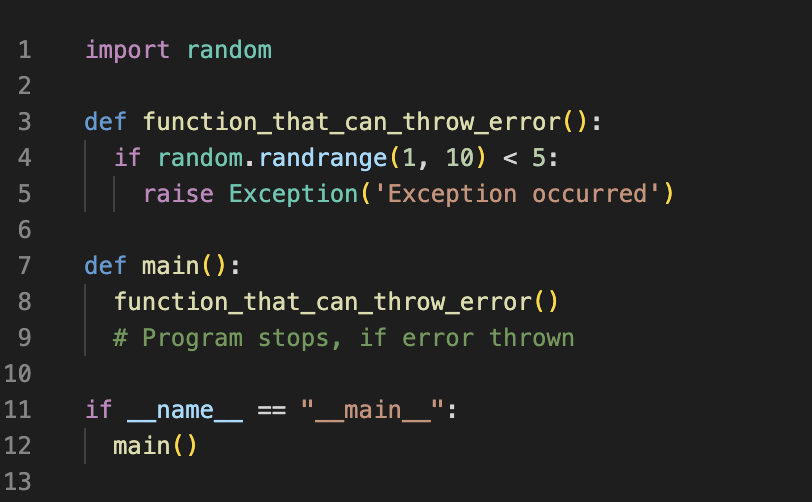
\includegraphics[width=5cm]{assets/noExceptionHandling.png}
      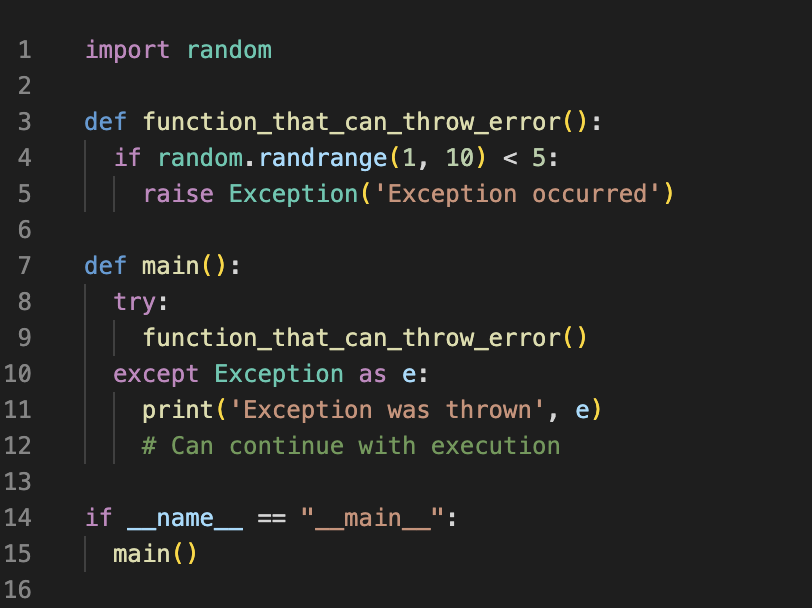
\includegraphics[width=5cm]{assets/exeptionHandling.png}
      \caption{Code demonstrating error handling (right) and no error handling (left) using Python.}
      \label{fig:errorHandling}
    \end{figure}

    \item \textit{Minimise the use of error-prone constructs} - A list of these constructs was compiled by Ian Somerville [34], however a lot of these
    are outdated, and refer to languages like C where memory allocation, array bound checking and pointers all posed issues for the developer when used
    incorrectly. A principle ACME follows is DRY code [35], which refers to clear concise code and Don't Repeat Yourself. Other issues are poor documentation.
    If everyone left the team then the new employees need this documentation to fully understand how the system works.

    \item \textit{Provide restart capabilities} - This is discussed in the \hyperref[sec:Rollbacks]{\textbf{Rollbacks}} section.

    \item \textit{Check array bounds} - 
    Memory leaks are no longer an issue in modern languages, but errors can still occur. Some languages like JavaScript allow this access and return a default 
    value instead of erroring. However this still has to be checked, otherwise functions that don't exists could be called, ending in system failure/error.

    \item \textit{Include timeouts when calling external components} - Long waits are frustrating for users but can also lead to system errors. If another 
    part of the ui/system is expecting data at a certain point this could lead to an error/fault in the system. Most libraries allow an option like this,
    however wherever this is not the case ACME has implemented their own timeouts and fallbacks.

    \item \textit{Name all constants that represent real-world values} - This is a good practice and is sometime referred to as \textit{'magic numbers'} [36].
    This can be troublesome when these hard-coded values are used in multiple places. ACME uses config files for these values that can then be imported 
    throughout the project. This makes the code easier to change and more readable.

    \begin{figure}[H]
      \centering
      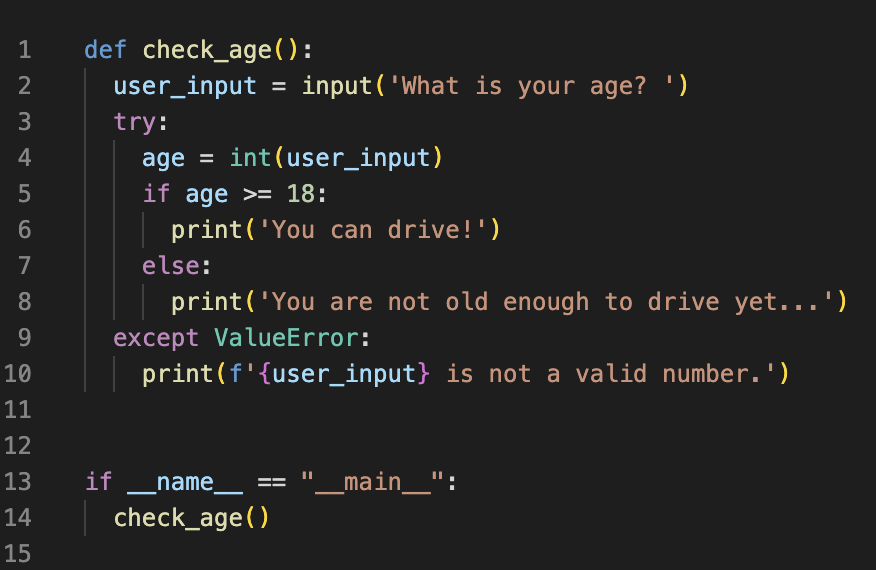
\includegraphics[width=5cm]{assets/magicNumbers.png}
      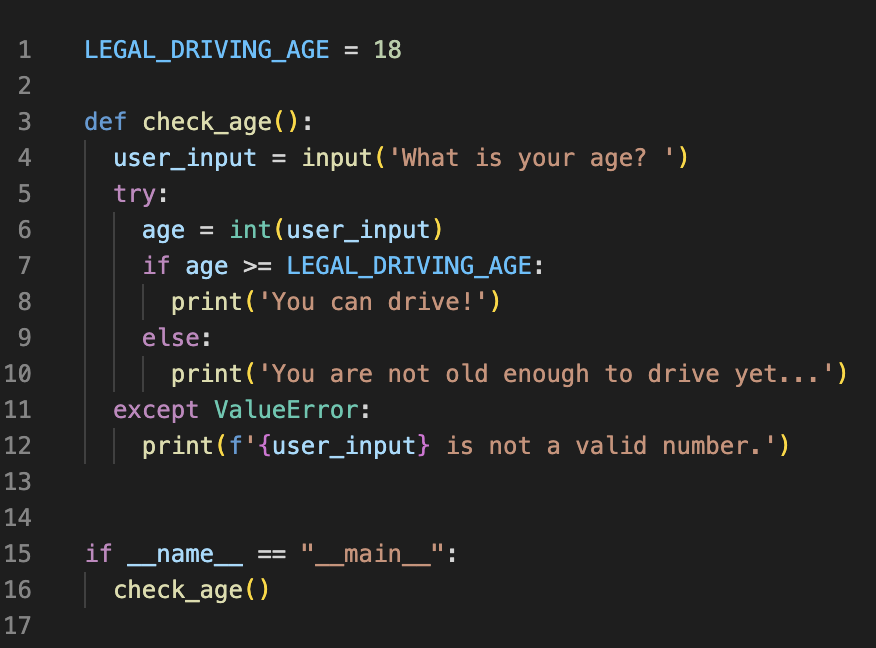
\includegraphics[width=5cm]{assets/noMagicNumbers.png}
      \caption{Code demonstrating magic numbers (left) and without (right) using Python.}
      \label{fig:magicNumbers}
    \end{figure}

  \end{enumerate}


  \subsubsection{Rollbacks}
  \label{sec:Rollbacks}
  AWS uses metrics to track events, these can be both default and custom metrics defined in code. These metrics can then be hooked up to alarms which 
  when state changes can trigger events that are handled by the EventBridge currently in the architecture [37]. These events can then be used to trigger
  additional actions such as code rollbacks or additional checks to determine/fix issues. ACME has a rollback procedure in place that is described and
  illustrated in \hyperref[sec:AppendixC]{\textbf{AppendixC}}.
  
  \subsection{Difference between safety and security threats}

  Safety and security are not the same things when it comes to software, a definition for safety is a:
  \begin{quote}
    \textit{'should never damage people or environment even though the system fails'}[38]
  \end{quote}

  Whereas security can described as:
  \begin{quote}
    \textit{'a system attribute that reflects the ability of the system to protect itself from external attacks, which may be accidental or deliberate.'} [38]
  \end{quote}

  Despite this there are situations in which these two can cross over fully. A german hospital was hacked and a woman ended up dying due the hack forcing her 
  to be transported to another hospital. This was deemed \textit{'the first known case of a life being lost as a result of a hack'} [39].

  \subsection{Safety}
  Safety of a system can often times be linked to harming other peoples health. The system ACME has created can't directly do that, however could have 
  indirectly. One issue is financial, a bug in the system could severely harm someone financially. There is also a chance cars provided 
  are faulty or the person driving them provided fake ID to gain access to the vehicle, then causing others harm.

  Lets starts by discussing financial issues, I previously talked about debouncing being a way to stop users accidentally performing an action more than
  once. Other ways include making sure a user has to confirm there purchase after the initial action can stop accidental purchases. However mistakes can 
  still happened, therefore ACME offers email and phone channels where customers can communicate with staff to get refunded.

  To verify drivers are who they say they are ACME has multiple checks before keys are given to a customer. The UK government offers a service to check 
  the validity of individuals driving licenses [40], which will be used when the customer creates an account. Adding further security to this, drivers licenses
  must be checked when the customer picks up the car. If something isn't correct, the customer is refunded and the car is not rented to them.

  The above actions help minimise the damage that can be done to ACMEs customer and products.

  \subsection{Security}
  I now will discuss security in two categories, physical (real-world) and software.

  \subsubsection{Physical}
  \vspace{0.2cm}
  Some threats of physical security are reduced due to the cloud-native approach chosen. This is due to no on-prem servers being used, therefore 
  user data is not accessible through ACME. However there are still some threats worth discussing.

  \begin{itemize}
    \item \textit{Tailgating} - This is a method where an \textit{'unauthorized person gains physical access to an off-limits location'} [41]. This can 
    lead this individual gaining access to machines or information they shouldn't have access to. Staff training is required here as well as tight security
    policies around passes. Gates should only allow one person through at a time and staff should report any suspicious behaviour.

    \item \textit{Physical access to machines} - This can be garnered by the above method or other methods of social engineering/distraction. This shouldn't
    be too hard to prevent, if devices like PCs are locked when the user is not there. In addition, ACME will have a password policy that makes sure that 
    passwords are changed every 3 months as well meet certain criteria, such as length and special characters contained. I don't recommend a password manager 
    despite their ease of use as this represents a single point of failure [42]. Tools like haveibeenpwned [43] can also be used to determine whether someones 
    email has been in a recent security breach.
  
  \end{itemize}

  \subsubsection{Software}
  I have spoke throughout this report about software security risks that can occur if developers are not careful. In this section I want to discuss
  more about preventative measures that ACME takes to avoid software issues from happening.

  \begin{itemize}
    \item \textbf{Penetration testing} - This \textit{'is a cyberattack simulation launched on your computer system'} [44] most often carried out by a
    third party. There are 3 different approaches to this, black, grey and white box [45].

    \begin{table}[H]
      \centering
      \begin{tabular}{|l|l|}
        \hline
        \textbf{Type} & \textbf{Access Granted}   \\ \hline
        Black Box     & None                      \\ \hline
        Grey Box      & Some                      \\ \hline
        White Box     & Full Access               \\ \hline
      \end{tabular}
      \caption{Table showing pen testers access using different methodologies.}
    \end{table}

    I would recommend a mixture of black and white box pen testing. Black box simulates an attacked on the outside trying to gain access to the system.
    Whilst a white box test gives the pen tester the chance to view the inner workings of the code. This could flag any potential vulnerabilities that 
    made it through the QA/testing phase. This should be done once a year, as these services can cost 
    \textit{'anywhere between £600 to over £3000 per day'} [46].

    \item \textbf{Principle of least privilege (PoLP)} - As previously \hyperref[sec:PoLP]{\textbf{menitioned}} ACME will incorporate processes for 
    both onboarding and off-boarding new staff members. No staff member should have any privileges they do not need to do their job. This can seem 
    untrusting, however with 34\% of businesses suffering attacks from insiders [47] and 66\% of companies being more worried about an internal attack 
    than a external attack [47] highlights the potential issue.

    \item \textbf{QA validation/testing} - The value of testing is discussed more in the \hyperref[sec:Testing]{\textbf{Testing}} section.
    
    \item \textbf{Code reviews} - Code reviews act as a \textit{'second opinion'} [48] on newly implemented code. Another developer should always read any 
    code that plans to be released to a live environment to help stop bugs reaching consumers.

    \item \textbf{Strict dependency selection} - ACME should use only well-known and tested external dependencies. In addition to this these should be checked
    into code so other developers can review them before live release. There have been multiple instances [49] where packages have been 
    \textit{'typo-squatted'} [50] and made their way to consumers.
    
    \item \textbf{Firewalls/blacklists} - AWS offers services such as WAF [51] to help protect customers against some forms of attacks. An extra layer can be 
    added to this. Software can be written to determine malicious or concerning usage of the web app, such as excessive requests (DDos) attack3[52]. 
    These can then be put onto a blacklist and their requests can be dropped from then on.
  \end{itemize}

\newpage
